\documentclass[conference]{IEEEtran}
\usepackage[dvips]{graphicx} 
\usepackage[tight]{subfigure}
\usepackage[numbers]{natbib}

\usepackage{url}
\usepackage{multirow}
\usepackage{array}
\usepackage{epsfig}
\usepackage{footnote}
\usepackage{amsmath}

\hyphenpenalty=10000
\tolerance=10000

\begin{document}

\title{Towards Social Profile Based Overlays}

\author{
David Isaac Wolinsky,
Pierre St. Juste,
P. Oscar Boykin,
Renato Figueiredo
\\
University of Florida
\\
}

\maketitle

\begin{abstract}

Online social networking has quickly become one of the most common activities
of Internet users.  As social networks evolve, they encourage users to share
more information, requiring the users, in turn, to place more trust into
social networks.  In centralized systems, this means trusting a third-party
commercial entity, like Facebook or MySpace, where as peer-to-peer (P2P)
systems can enable the creation of online social networks where trust need
only be extended to friends.  In this paper, we present a novel approach to
constructing completely decentralized social networks.  All users join a
common directory overlay, which facilitates friend discovery connecting peers
to individualized profile overlays, mapping the ownership of the overlay to
the ownership of the profile.  Each user transparently manages access to their
profile through the use of a public key infrastructure (PKI).  We define
interfaces and present tools that can be used to implement this system, as
well.  The key aspects of P2P as it applies to this work include
self-organization, self-configuration, and scalability.

\end{abstract}

\section{Introduction}

Online social networking has become pervasive in daily life, though as social
networks grow so does the wealth of personal information that they store.
Once information has been released on a social network, known as a user's
profile, the data and the user are at the mercy of the terms dictated by the
social network infrastructure, which today is typically third-party, centrally
owned.  If the social network engages in activities disagreeable to the user,
due to change of terms or opt-out programs not well understood by users such
as recent issues with Facebook's Beacon program~\cite{facebook_beacon}, the
options presented to the user are limited: to leave the social network
(surrendering their identity and features provided by the social network), to
accept the disagreeable activities, or to petition and hope that the social
network changes its behavior. 

As the use of social networking expands to become the primary way in which
users communicate and express their identity amongst their peers, the users
become more dependent on the policies of social network infrastructure owners.
Recent work~\cite{p2p_socialnetwork} explores the coupling between social
networks and P2P systems as a means to return ownership to the users, noting
that a social network made up of social links is inherently a P2P system with
the aside that they are currently developed on top of centralized systems.  In
this paper, we extend this idea with focus on the topic of topology; that is,
how to self-organize social profiles that leverage the benefits offered by a
structured P2P overlay abstraction.

Structured P2P overlays provide a scalable, resilient, and self-managing
platform for distributed applications.  Structured overlays enable users to
easily create their own decentralized systems for the purpose of data sharing,
interactive activities, and other networking-enabled activities.  In this
paper, we extend our previous work~\cite{vpo} to enable social network profile
overlays.  The previous work addresses the challenges of bootstrapping secure,
private overlays in NAT and firewall environments by using a public overlay
for discovery and as a relay or communication transport.  

Social networks consist of users and groups.  Each user has a profile, a set
of friends, and private messaging; while each group consists of one or more
managers, users, and a messaging board.  The profile contains user's personal
information, status updates, and public conversations, similar to a message
board.  Friends are individuals trusted sufficiently by a user to view the
user's profile.  Private messaging enables sending messages discretely between
users without leaking the message to other members.  A group is very similar
to an individual profile, though it is shared by many users.  In some cases,
groups are open, though others require approval from an administrator, and in
general all users can post messages to the group.  

Using this social networking model, we describe how a public overlay can be
used as a directory for finding and befriending friends or finding and
accessing groups.  Once access has been enabled, the public overlay can be used
to bootstrap connectivity to existing profile and group overlays.  Security for
profile are provided by a public key infrastructure (PKI), where profile owners
or group managers are the certificate authorities (CA) and all members have
signed certificates.  The overlay stores profile data or group information in
its distributed data store, supporting decentralized access using scalable
mechanisms regardless of the profile owner's online presence.  In this paper,
we present the architecture of these overlays, as presented in
Figure~\ref{fig:system}.

\begin{figure}[h]
\centering
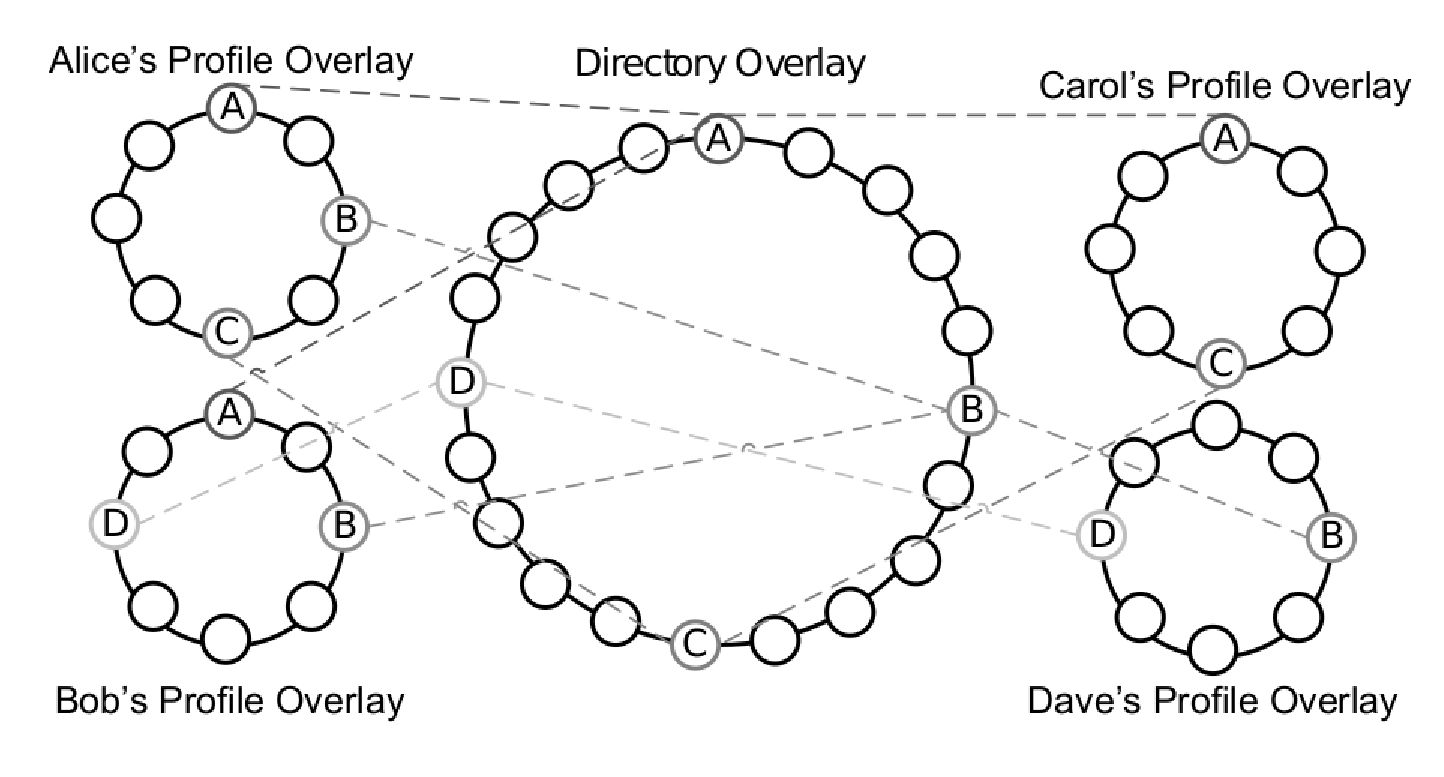
\epsfig{file=figs/subrings.eps, width=3.12in}
\caption{An example social overlay network.  Alice has a friendship with Bob
and Carol, hence both are members of her profile overlay. Bob has a friendship
with Alice and Dave but not Carol; hence Alice and Dave are members of his
profile overlay, while Carol is not.  Each peer has many overlay memberships
but a single root represented by dashed lines in various shades of gray.  For
clarity, overlay shortcut connections are not shown.} \label{fig:system}
\end{figure}

The rest of this paper is organized as follows.  Section~\ref{background}
provides background and related work.  Section~\ref{social_overlays} describes
our multi-overlay approach, explaining how to map social networks onto
structured P2P overlays.  In Section~\ref{outstanding}, we explore some of the
remaining challenges introduced by our approach.  We conclude the paper in
Section~\ref{conclusion}.

\section{Background}
\label{background}

In this section, we review structured P2P overlays, challenges and solutions
for bootstrapping overlays, and other methods for constructing decentralized
online social networks.  We place an early emphasis on structured P2P systems,
as they  provide the basis for our approach by  creating scalable, autonomic
environments, thereby limiting user exposure to the gory details of system
configuration and organization.  Though P2P systems can be difficult to
bootstrap especially when their are no dedicated bootstrapping nodes.

\subsection{Structured P2P Overlays}

There are two types of P2P systems, unstructured and structured.  Unstructured
systems are generally constructed by peers attempting to maintain a certain
amount of connections to other peers in the P2P system, whereas structured
systems organize into well-defined topologies, such as 2-D rings or
hypercubes.  Though unstructured systems are typically simpler to bootstrap
and maintain, they rely on global knowledge, flooding, or stochastic
techniques to search for information in an overlay and thus have scalability
constraints.  Alternatively, structured systems have guaranteed search time
typically with a lower bound of $O(\log N)$.  Some examples of structured
systems are Pastry~\cite{pastry}, Chord~\cite{chord},
Symphony~\cite{symphony}, Kademlia~\cite{kademlia}, CAN~\cite{can}, and
Dynamo~\cite{dynamo}.

A key component of most structured overlays is support for decentralized
storage / retrieval of information by mapping keys to specific node IDs in an
overlay called a distributed hash table (DHT).  At a minimum, the data is
stored at the node ID either smaller or larger to the data's node ID and for
fault tolerance the data can be stored at other nodes.  DHTs can be used by
peers of systems to coordinate allocation and discovery of resources, making
them attractive for self-configuration in decentralized collaborative
environments.  DHTs provide the building blocks to form more complex
distributed data stores as presented in Past~\cite{past} and
Kosha~\cite{kosha}.

\subsection{Bootstrapping P2P Overlays}

One of the key challenges to overlays is the bootstrapping problem, that is,
ho do I find an active member in the overlay so that I can be a contributing
member of the overlay.  In large public systems, often times, the owners of
the project and sometimes corporate sponsors provide these resources, though
these types of bootstrapping peers are typically not available for small,
private overlays.  The bootstrapping problem can be divided into two
components: finding a bootstrapping member of the overlay and handling
connectivity constraints if the overlay has no members with public addresses.
In~\cite{one_ring, can_multicast}, the authors discuss the concept of a single
overlay supporting services through the use of additional overlays, which use
the underlying overlay to assist in discovery, this deals with the component
of finding a bootstrap peer.  To address the challenge of bootstrapping peers
being behind NATs, we described a system in~\cite{vpo} enables the public
overlay to act as a NAT traversal rendezvous point.  More specifically, a
peer, attempting to join a private overlay, queries the public overlay's DHT
to obtain a list of currently online private overlay peers who have matching
public IDs.  The peers then use the public overlay, in addition to direct UDP
or TCP links, to communicate with the private overlay nodes and bootstrap into
the private overlay.  This method enables peers even behind firewalls and NATs
to have publicly available addresses in the public overlay.  Additionally this
work describes mechanisms that enable the use of PKI technologies to
seamlessly secure both point-to-point and end-to-end communication in a
structured overlay.

During evaluation, using both simulated and real systems, the time for a
single peer to join first the public and thereafter private overlays was small
and grew logarithmically with network sizes.  The real system was tested using
a public overlay of 600 nodes on PlanetLab and a random distribution of peers
in the private overlay.  With point-to-point security links enabled in the
private overlay, the time to connect was less than 22 seconds for all cases.
In simulations, overlays with as many as 100,000 peers were evaluated.  For
the 100,000-peer overlay, regardless of the private overlay size and with
security enabled, peers were able to connect to their private overlays in less
than 48 seconds.  In relation to this paper, these results can be interpreted
such that the latency required for a single peer to from being completely
disconnected from the social network to being fully connected to the directory
and all profile overlays.

\subsection{Peer-to-Peer Social Networks}

In~\cite{peerson}, a DHT provides the look-up service for storing meta data
pertaining to a peer's profile.  Peers query the DHT for updated content from
their friends by hashing their unique identifiers (e.g. friends' email
addresses).  The retrieved meta data contains information for obtaining the
profile data such as IP address and file version. Their work relies on a PKI
system that provides identification, encryption, and access control.  In
contrast, our approach provides each user their own private overlay secured by
point-to-point encryption and authentication amongst all peers in the profile
overlay.  The profile overlay provides a clean abstraction of access control,
whereby once admitted to a private overlay, users can access a distributed
data store which holds the contents of the owners profile.

\cite{vis-a-vis} takes a different approach by depending on virtual individual
servers (VIS) hosted on a cloud infrastructure such as Amazon EC2. Friends
contact each other's VIS directly for updates.  A DHT is used as a directory
for groups and interest-based searches. Their approach assumes bidirectional
end-to-end connectivity between each VIS, where a profile is only available
during the up time of the VIS.  Because of the demands on network connectivity
and up time, the approach assumes a cloud-hosted VIS and has difficulty being
used on user-owned resources.  Our approach enables users to avoid the need
for all-to-all connectivity and constant up time through the use of NAT
traversal support and the ability to store the profile in the overlay's
distributed data store.

The approach presented in~\cite{matryoshka} relies on a central system to host
identities and certificates that can then be used to query a DHT to discover
an initial hop in a route to a specific peer through their circle of friends.
The circle of friends consists of an unstructured overlay, where direct
friends maintain direct connections with the peer, and outer circles consist
of friends of friends and friends of friends of friends.  The main goal of
this work is to remove the private components of a profile from a central
entity, whereas our approach makes a clean break from all centralization and
emphasizes scalability through distributed replica techniques.

Unlike the above approaches, the P2P social network presented
in~\cite{tribler-osn} uses an unstructured overlay without a DHT where peers
connect directly to each other rather than through the overlay establishing
unique identifiers to deal with dynamic IPs.  Peers cache each other's data to
improve availability.  While helper nodes are used to assist with
communication between peers behind NATs.  The approach lacks security and
access control considerations and lacks the guarantees and the simplicity of
the abstraction offered by a structured overlay.

\section{Social Overlays}
\label{social_overlays}

In this section, we explain how to map online social networking to virtual
private overlay based social network consisting of a public directory overlay
with many private profile overlays.  The directory overlay supports friend
discovery and verification and stores a lists of peers currently active in
each profile overlay.  Profile overlays support message boards, private
messages, and media sharing.

\subsection{Finding and Verifying Friends}

In a traditional social network, a directory provides the ability to search
for users using public information, such as the user's full name, user ID,
e-mail address, group affiliations, and friends.  The search results return
zero or more matching directory entries.  Based upon the results, the user,
\textit{A}, can potentially make a friendship request.  The request receiver,
\textit{B}, can review the public information of A to making a decision.  If
\textit{B} accepts the request, \textit{A} and \textit{B} are given access to
each other's profiles.  Once profile access has been enabled, the users can
learn more information, and if it turns out to be a mistake, the peers can
unilaterally end the relationship.

One method to map this to our proposed social overlay would be for directory
entries to be inserted into the DHT of a public overlay.  A user could store
their public information at a single location in the DHT, which would be
indexed through multiple mappings involving their public information.  For
example, a user could store at the DHT key $hash("alice")$ or $hash("alice
bob")$ a pointer to the DHT location for their certificate.  The key here is
that any subset of the user's public information in lower-case format could be
hased into an index into the DHT that would eventually direct the searching
user to one or more user's certificates.  Public information should consist of
as much identifiable information the peer is willing to share and an overlay
address.  The overlay address enables asynchronous offline messaging, such as
friendship requests, which will be explained shortly.

Because the users need a way to verify each other that involves social
credentials, we propose the use of a new form of certificate.  The main
portion of the certificate is similar to a self-signed x509 certificate with
public information such as user's name, e-mail address, and group affiliations
embedded into the certificate.  At the tail of the certificate is a friend
list represented by many friend entries.  To do this we propose employing a
technique similar to PGP: users can acquire from their friends a signed
message consisting of a hash of the peer's certificate, the time stamp, and
the friend's certificate hash signed by the friend.  Since PGP does not
provide a strong method for revocation, the time stamp provides additional
information to help decide whether or not a friendship link is still active
without accessing the profile overlay of either peers.  Peers should request a
new friend list entry within a certain period of time or it will appear that
the friendship is no longer valid.

While looking for an individual, a peer may discover that many individuals
have overlapping public information components, such as the user's name.
Assuming all entries are legitimate, the overlay must have some method of
supporting multiple, distinct values at the same key, leaving the peer or the
peer's DHT client to parse the responses and determining the best match by
reviewing the contents of each certificate.  Alternatively, a technique like
Sword~\cite{sword}, which supports distributing the data across a set of nodes
and using a bounded broadcast to discover peers that match all information,
could be used for searching.

If a peer, \textit{A}, desires a friendship with another peer, \textit{B},
\textit{A} issues a friendship request, which will be stored in the DHT at the
overlay address listed in \textit{B}'s certificate, as described earlier.  The
friendship request consists of the self-signed certificate of \textit{A}, the
requesting peer; the public information of the request receiver, \textit{B};
and a time stamp; all signed with the private key associated with \textit{A}'s
private key matched to their self-signed certificate.

Within a reasonable amount of time after a request has been inserted into the
DHT, \textit{B} can come online and check for outstanding requests.  Upon
receiving a request, \textit{B} has three choices: a conditional accept, an
unconditional accept, or a reject.  During an unconditional accept, \textit{B}
signs \textit{A}'s request and issues a request to befriend \textit{A}.
Alternatively in the case of a conditional accept, \textit{B} issues a
friendship request, waits for a reply, and investigates the profile prior to
signing the \textit{A}'s request.  Once a user has received a signed
certificate, they may access the remote peer's profile overlay as discussed
in~\ref{profile_overlay}, which is also responsible for activities such as
revocation.

\subsection{The Profile Overlay}
\label{profile_overlay}

In a traditional social network, the profile or user-centric portion consists
of private messaging, data sharing, friendship maintenance, and a public
message board for status updates or public messages.  In this section, we
explain how these components can be applied to a structured overlay dedicated
to an individual profile.

Using the techniques such as those described in~\cite{vpo}, it is feasible to
efficiently multiplex a P2P system across multiple, virtual private overlays
enabling each profile owner to have a profile overlay consisting of their
online friends.  For access control, we employ a PKI, where each member uses
the signed certificate generated during the ``finding and verifying friends''
stage.  All links are encrypted using symmetric security algorithms
established through the PKI, thus preventing uninvited guests from gaining
direct access to the overlay and hence the profile.  Because the profile owner
also is the CA for all members of the overlay, they can easily revoke users
from access to the profile overlay.  In~\cite{vpo} describes efficient
mechanisms for overlay revocation through the use of broadcasting for
immediate revocation and the use of DHT for indirect and permanent revocation.

The message board of a profile can be stored in two ways: distributed within
the profile overlay via a data store or stored on the profile owner's personal
computing devices.  The distributed data store provide the profile when the
owner is offline and also distributes the load for popular profiles.  For
higher availability, each peer should always be a provider for all data in
their profile when they are online.  To ensure authenticity and integrity, all
peers should sign their messages and each peer's certificate should be
available in the overlay for verification.  Messages that are unsigned should
be ignored by all members of the overlay.  An ideal overlay for this purpose
should support complex queries~\cite{complex_queries} allowing easy access to
data stored chronologically, by content, by type, i.e., media, status updates,
or message board discussions.

Private messaging in the profile overlay is unidirectional meaning that only
the profile owner can receive private messages using their overlay.  To
enforce this, a private message should be prepended with a symmetric key
encrypted by the profile owners public key, the message should be appended by
a hash of the message to ensure integrity and the entire message encrypted by
the symmetric key.  This approach ensures that only the sender and the profile
owner can decrypt the private message.  The contents of the private message
should include the sender, time sent, and the subject.  Messages can be stored
in well known locations, so that the profile owner can either poll the
location or, alternatively, use an event based system to notify them of the
new message.

\subsection{Event Based Message Notification}

Both the directory and profile overlays have methods by which peers can receive
messages.  In the directory overlay, these take form by means of friendship
request and accept.  In the profile overlay, they consist of private messages.
While polling the location in the DHT occasionally will allow peers to
receive the messages, polling has inherent delays and network costs.
Alternatively, an event mechanism would enable peers to receive sent messages
very quickly after they have been sent with minimal impact on network
throughput.

A simple method for implementing an event notification system involves using
the DHT.  Each event would have an identification that would map to a list of
peers wanting to know when an event occurred and the data associated with it.
Thus mapping the $(event id, listener)$ to the DHT could be done by hashing a
string such as ``private messages for me'' and storing the profile owners
active nodes into the list of listeners.  When a message was stored to the
users mailbox, the sender could query this list and send to each listener a
notification of the new private message.  Alternatively, if a higher degree of
anonymity is required, the DHT server could be modified to forward the
response to the listeners directly rather than returning a list of listeners.
Of course, this does not prevent potential race conditions occurring, such as
a situation where a peer recently joined their profile overlay, had already
queried their mailbox and found it empty, while simultaneously a private
message was sent to them yet they were not in the listeners list.  Thus
occasional polling is required, though can be minimized, the longer a node
has been online.

\subsection{Active Peers}

The directory overlay should be used to assist in finding currently active
peers in the profile overlays.  By placing their node IDs at a well-known,
unique per-profile overlay keys in the DHT, active peers can bootstrap
incoming peers into the profile overlay.  We implemented and evaluated this
concept in~\cite{vpo}.  Because the profile overlay members all use PKI to
ensure membership, even if malicious peers insert their ID into the active
list, it would be useless as the peer would only form connections with peers
who also have a signed certificate.

\subsection{Groups}

Groups can be considered extensions of profile overlays.  The fundamental
difference between a group and a profile is that a group lacks private
messaging and has shared ownership.  So just as a peer can find a profile in
the directory by hashing the name of the user and other identifiable
information, so can the user find the group.  Like the certificate of the
user, the members of a group sign the groups certificate to represent their
membership to that group.  The user requests membership to the group and a
group manager can sign the certificate allowing that member access to the
group.  Finally, the group can be bootstrapped in the same way as the profile
overlay through the directory overlay.

The unique challenge presented by groups is the sharing of the CA task.  A
decentralized solution would be for all members of the group to be listed in
the groups DHT and when a peer becomes a manager, their certificate is added
to the certificate chain for the group enabling them to sign certificates for
that group.  If an administrator loses their position, then all members who
had their certificate signed by that administrator would need to obtain a new
certificate.  Alternatively, the owner of the group and the original CA could
sign the group members certificates again, so that they are signed by the root
CA and would not lose access if administration changes.

\section{Challenges}
\label{outstanding}

While structured P2P overlays have been well-studied in a variety of
applications, their use in social profile overlays raises new interesting
questions, including:

{\bf 1) Handling small overlay networks} - P2P overlay research typically
focuses on networks larger than the typical user's friend count (Facebook's
average is 130\footnote{http://www.facebook.com/press/info.php?statistics}).
Because social profile overlays are comparatively smaller, this can impact the
reliability of the overlay and availability of profile data.  A user can host
their own profile; however when the user is disconnected it is important that
their profile remains available even under churn. It is thus important to
characterize churn in this application to understand how to best approach this
problem. An optional of per-user deployment of a virtual individual server
(VIS) and the use of replication schemes aware of a user's resources provide
possible directions to address this issue.

{\bf 2) Overlay support for low throughput, unconnected devices} - devices such
as smart phones cannot constantly be actively connected to the overlay and the
connection time necessary to retrieve something like a phone number may be too
much to make this approach useful.  Similar to the previous challenge, this
approach could benefit from using a VIS enabling users access to their social
overlays by proxy without establishing a direct connection to the overlay
network.

{\bf 3) Reliability of the directory and profile overlay} - Overlays are
susceptible to attacks that can nullify their usefulness.  While the profile
overlay does have point-to-point security, in the public, directory overlay,
the lack of any form centralization makes policing the system a complicated
procedure.  While our approach of appending friends list can assist users in
making decisions on identity, it does not protect against denial of service
attacks.  For example, users could attempt create many similar identities in
an attempt to overwhelm a user in their attempt to find a specific peer.
Previous work has proposed methods to ensure the usability of overlays even
while under attack.  For the social overlay to be successful, we must identify
which methods should be used. A possible approach is to replicate public
information within a user's profile overlay thus providing an alternative
directory overlay for querying prior to using the public directory overlay.

\section{Conclusion}
\label{conclusion}

In this paper, we proposed methods by which a social network can be
decentralized through the use of structure P2P overlays.  P2P systems, in
general, have very nice properties that make them attractive for average
users.  Namely, they require minimal configuration and organization of
resources, in addition, P2P systems naturally handle increased demand to
additional peers.  Our approach is based upon the use of a multiple overlay
system, where all users join a public directory overlay and their's as well as
their friends profile overlays.  The directory overlay enables users to find
and befriend other peers and bootstrap connections into the secure profile
overlays.  Upon forming a friendship through the directory overlay, peers are
given CA signed certificates that allow them to join each other's profile
overlay.  The owner of the profile overlay acts as CA enabling unilateral
dismissal of friendships via certificate revocation using efficient and
reliable methods.  For the purpose of storing profile information into the
overlay, we cite previous work that can be used to provide distributed data
services and give examples of how to store data securely in the overlay.  Our
proposed system returns control of the social network and more importantly
users' identity to the users and eliminates the need for centralized social
networks.

\small{
\bibliographystyle{IEEEtran}
\bibliography{SocialProfileOverlays}
}

\end{document}
